\documentclass{article}
\usepackage{xcolor}
\usepackage[paperheight = 16in, paperwidth = 7in, margin = 0.5in]{geometry}
\usepackage{tikz} 
\renewcommand{\familydefault}{\sfdefault}
\usetikzlibrary{calc, shapes, matrix, arrows, positioning}
% Create some types of boxes and arrows:
% for loop (red)
% a process (green)
% an if statement (blue)
% and an arrow.

\tikzstyle{forloop} = [rectangle,
                       rounded corners,
                       minimum width = 1cm,
                       minimum height = 1cm,
                       line width = 0.5mm,
                       text centered,
                       text width = 4cm,
                       draw = gray,
                       fill = red!20]

\tikzstyle{process} = [rectangle,
                       rounded corners,
                       minimum width = 1cm,
                       minimum height = 1cm,
                       line width = 0.5mm,
                       text centered,
                       text width = 4cm,
                       draw = gray,
                       fill = green!20]

\tikzstyle{if} = [rectangle,
                  rounded corners,
                  minimum width = 1cm,
                  minimum height = 1cm,
                  line width = 0.5mm,
                  text centered,
                  text width = 4cm,
                  draw = gray,
                  fill = blue!20]

\tikzstyle{arrow} = [rounded corners, thick,->,>=stealth]

\begin{document}
% Turn off page numbering on this page.
\thispagestyle{empty}
\begin{center}
\scalebox{0.55}{

% Create a massive vectorised picture!
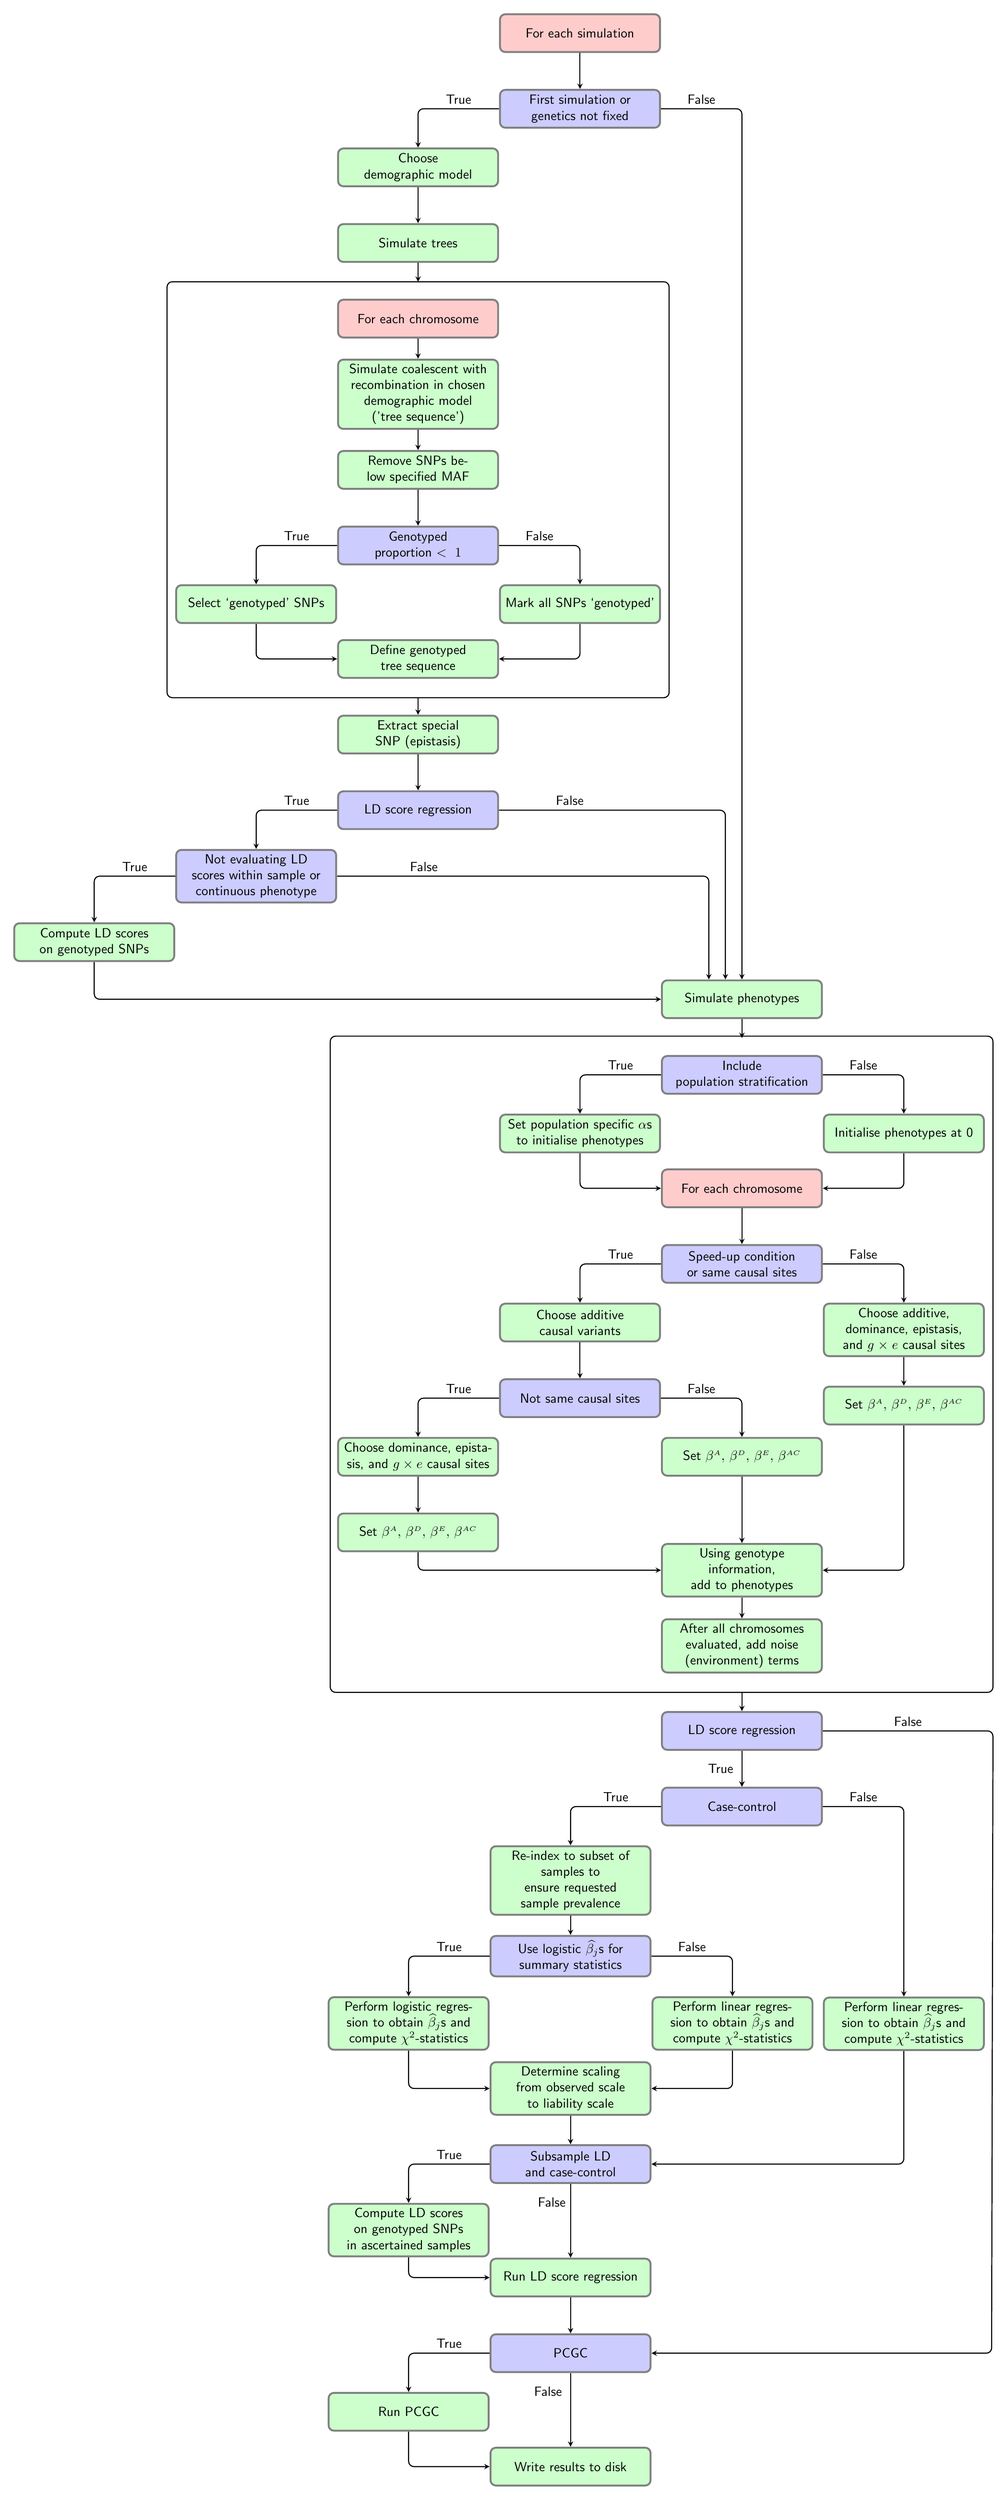
\begin{tikzpicture}[node distance=2cm]

% First set of nodes.
\node (foreachsim) [forloop]
{For each simulation};

\node (fixedgen) [if, below of=foreachsim]
{First simulation or genetics not fixed}; 

\node (choosedemmodel) [process, below left=0.5cm and 0cm of fixedgen]
{Choose \\demographic model};

% Nodes for tree simulation - to be put in a box.
\node (simtrees) [process, below of=choosedemmodel]
{Simulate trees};

\node (foreachchr) [forloop, below of=simtrees]
{For each chromosome};

\node (simatree) [process, below of=foreachchr]
{Simulate coalescent with recombination in chosen demographic model\\('tree sequence')};

\node (maf) [process, below of=simatree]
{Remove SNPs below specified MAF};

\node (genoprop) [if, below of=maf]
{Genotyped\\proportion $<1$};

\node (genopropt) [process, below left=0.5cm and 0 cm of genoprop] {Select `genotyped' SNPs};

\node (genopropf) [process, below right=0.5cm and 0 cm of genoprop] {Mark all SNPs `genotyped'};

\node (genotreeseq) [process, below of=simtrees, yshift = -9cm] {Define genotyped tree sequence};

% Add in the arrows.
\draw [arrow] (genoprop) -| node[anchor=south, near start] {True} (genopropt);
\draw [arrow] (genoprop) -| node[anchor=south, near start] {False} (genopropf);
\draw [arrow] (genopropt) |- (genotreeseq);
\draw [arrow] (genopropf) |- (genotreeseq);
\draw [arrow] (simatree) -- (maf);
\draw [arrow] (maf) -- (genoprop);
\draw [arrow] (foreachsim) -- (fixedgen);
\draw [arrow] (fixedgen) -| node[anchor=south, near start] {True} (choosedemmodel);
\draw [arrow] (foreachchr) -- (simatree);
\draw [arrow] (choosedemmodel) -- (simtrees);

% Create box around the tree simulation.
\draw [rounded corners, thick] ($(genotreeseq.south west)+(-4.5cm,-0.5cm)$) rectangle ($(genotreeseq.south east)+(4.5cm,10.5cm)$);
% \node[left of=foreachchr, xshift=-2cm, align=left, text width=4cm, font=\Large]{Simulate trees};

% Potential evaluation of LD scores before computing phenotypes.
\node (epi) [process, below of=genotreeseq]
{Extract special SNP (epistasis)};

\node (ldsc) [if, below of=epi]
{LD score regression};

\node (fullsampleornotcasecontrol) [if, below left=0.5cm and 0cm of ldsc]
{Not evaluating LD scores within sample or continuous phenotype};

\node (ldscores) [process, below left=0.5cm and 0 cm of fullsampleornotcasecontrol]
{Compute LD scores on genotyped SNPs};

\node (phenotypes) [process, below right=22.5cm and 0cm of fixedgen]
{Simulate phenotypes};

% Add in the arrows.
\draw [arrow] (fullsampleornotcasecontrol) -| node[anchor=south, near start] {True} (ldscores);
\draw [arrow] (ldsc) -| node[anchor=south, near start] {True} (fullsampleornotcasecontrol);
\draw [arrow] (epi) -- (ldsc);
\draw [arrow] ($(genotreeseq.south)+(0cm,-0.5cm)$) -- (epi);
\draw [arrow] (simtrees) -- ($(simtrees.south)+(0cm,-0.5cm)$);
\draw [arrow] (ldsc) -| node[anchor=south, near start] {$\hskip-2.25cm$False} ($(phenotypes.north)+(-0.4375cm,0cm)$);
\draw [arrow] (ldscores) |- node[anchor=east] {} (phenotypes);
\draw [arrow] (fullsampleornotcasecontrol) -| node[anchor=south, near start] {$\hskip-5.25cm$False} ($(phenotypes.north)+(-0.875cm,0cm)$);
\draw [arrow] (fixedgen) -| node[anchor=south, near start] {False} (phenotypes);

% Phenotype evaluation.
\node (popstrat) [if, below of=phenotypes]
{Include\\population stratification};

% \node[left of=popstrat, xshift=-5cm, align=left, text width=6cm, font=\Large]{Simulate phenotypes};

\node (popstratt) [process, below left=0.5cm and 0 cm of popstrat]
{Set population specific $\alpha$s to initialise phenotypes};

\node (popstratf) [process, below right=0.5cm and 0 cm of popstrat]
{Initialise phenotypes at 0};

\node (foreachchr2) [forloop, below of=popstrat, yshift = -1cm]
{For each chromosome};

\node (speedup) [if, below of=foreachchr2]
{Speed-up condition or same causal sites};

\node (addcausal) [process, below left=0.5cm and 0 cm of speedup]
{Choose additive causal variants};

\node (samecausal) [if, below of=addcausal]
{Not same causal sites};

\node (beta2) [process, below right=0.5cm and 0 cm of samecausal]
{Set $\beta^{\scriptscriptstyle A},\, \beta^{\scriptscriptstyle D},\, \beta^{\scriptscriptstyle E},\, \beta^{\scriptscriptstyle AC}$};

\node (decausal) [process, below left=0.5cm and 0 cm of samecausal]
{Choose dominance, epistasis, and $g\times e$ causal sites};

\node (beta) [process, below of=decausal]
{Set $\beta^{\scriptscriptstyle A},\, \beta^{\scriptscriptstyle D},\, \beta^{\scriptscriptstyle E},\, \beta^{\scriptscriptstyle AC}$};

\node (choosecausal) [process, below right=0.5cm and 0cm of speedup]
{Choose additive,\\ dominance, epistasis, and $g\times e$ causal sites};

\node (beta3) [process, below of=choosecausal]
{Set $\beta^{\scriptscriptstyle A},\, \beta^{\scriptscriptstyle D},\, \beta^{\scriptscriptstyle E},\, \beta^{\scriptscriptstyle AC}$};

\node (addtopheno) [process, below of=beta2, yshift=-1cm]
{Using genotype\\information,\\add to phenotypes};

\node (addnoise) [process, below of=addtopheno]
{After all chromosomes evaluated, add noise (environment) terms};

% Add in more arrows.
\draw [arrow] (addtopheno) -- (addnoise);
\draw [arrow] (foreachchr2) -- (speedup);
\draw [arrow] (speedup) -| node[anchor=south, near start] {True} (addcausal);
\draw [arrow] (addcausal) -- (samecausal);
\draw [arrow] (samecausal) -| node[anchor=south, near start] {False} (beta2);
\draw [arrow] (samecausal) -| node[anchor=south, near start] {True} (decausal);
\draw [arrow] (decausal) -- (beta);
\draw [arrow] (choosecausal) -- (beta3);
\draw [arrow] (speedup) -| node[anchor=south, near start] {False} (choosecausal);
\draw [arrow] (popstrat) -| node[anchor=south, near start] {True} (popstratt);
\draw [arrow] (popstrat) -| node[anchor=south, near start] {False} (popstratf);
\draw [arrow] (popstratt) |- (foreachchr2);
\draw [arrow] (popstratf) |- (foreachchr2);
\draw [arrow] (beta) |- (addtopheno);
\draw [arrow] (beta2) -- (addtopheno);
\draw [arrow] (beta3) |- (addtopheno);

% Create box around the phenotype simulation.
\draw [rounded corners, thick] ($(addnoise.south west)+(-8.75cm,-0.5cm)$) rectangle ($(foreachchr2.north east)+(4.5cm,3.5cm)$);

% Moving in to running LD score regression.
\node (ldscoretf) [if, below of=addtopheno, yshift=-2.25cm]
{LD score regression};

\node (casecontrol) [if, below of=ldscoretf]
{Case-control};

\node (ascertain) [process, below left=0.5cm and 0.25 cm of casecontrol] {Re-index to subset of\\samples to \\ensure requested\\sample prevalence};

\node (ldscnonlinear) [if, below of=ascertain]
{Use logistic $\widehat{\beta_j}$s for summary statistics};

\node (nonlinearchi) [process, below left=0.5cm and 0cm of ldscnonlinear]
{Perform logistic regression to obtain $\widehat{\beta}_j$s and compute $\chi^2$-statistics};

\node (chisqlin) [process, below right=0.5cm and 0cm of ldscnonlinear]
{Perform linear regression to obtain $\widehat{\beta}_j$s and compute $\chi^2$-statistics};

\node (chisq) [process, below right=4.5cm and 0cm of casecontrol]
{Perform linear regression to obtain $\widehat{\beta}_j$s and compute $\chi^2$-statistics};

\draw [arrow] ($(ldscoretf.north)+(0cm,0.5cm)$) -- (ldscoretf);
\draw [arrow] (ldscoretf) -- (casecontrol);
\draw [arrow] (casecontrol) -| node[anchor=south, near start] {True} (ascertain);
\draw [arrow] (ascertain) -- (ldscnonlinear);
\draw [arrow] (ldscnonlinear) -| node[anchor=south, near start] {True} (nonlinearchi);
\draw [arrow] (casecontrol) -| node[anchor=south, near start] {False} (chisq);
\draw [arrow] (ldscnonlinear) -| node[anchor=south, near start] {False} (chisqlin);
\draw [arrow] (phenotypes) -- ($(phenotypes.south)+(0cm,-0.5cm)$);

\node (scalinglog) [process, below of=ldscnonlinear, yshift = -1.5cm]
{Determine scaling from observed scale to liability scale};

\node (subsampleandcasecontrol) [if, below of=scalinglog]
{Subsample LD and case-control};

\draw [arrow] (nonlinearchi) |- (scalinglog);
\draw [arrow] (chisqlin) |- (scalinglog);
\draw [arrow] (scalinglog) -- (subsampleandcasecontrol);

\node (ldscore2) [process, below left=0.5cm and 0cm of subsampleandcasecontrol]
{Compute LD scores on genotyped SNPs in ascertained samples};

\node (reg) [process, below of=subsampleandcasecontrol, yshift=-1cm]
{Run LD score regression};

% Add in arrows.
\draw [arrow] (subsampleandcasecontrol) -| node[anchor=south, near start] {True} (ldscore2);
\draw [arrow] (subsampleandcasecontrol) -- node[anchor=east, near start] {False} (reg);
\draw [arrow] (ldscore2) |- (reg);
\draw [arrow] (chisq) |- (subsampleandcasecontrol);

% The PCGC portion of the code.
\node (pcgc) [if, below of = reg]
{PCGC};

\node (runpcgc) [process, below left=0.5cm and 0 cm of pcgc]
{Run PCGC};

\node (write) [process, below of=pcgc, yshift=-1cm]
{Write results to disk};

% Add in arrows.
\draw [arrow] (reg) -- (pcgc);
\draw [arrow] (pcgc) -- node[anchor=east, near start] {False$\;$} (write);
\draw [arrow] (runpcgc) |- (write);
\draw [arrow] (pcgc) -| node[anchor=south, near start] {True} (runpcgc);
\draw [arrow] (ldscoretf) -| node[anchor=south, near start] {False} ([shift={(4.5cm,0cm)}]ldscoretf.south east)-- ([shift={(9cm,0cm)}]pcgc.north east)|-(pcgc);
\draw [arrow] (ldscoretf) -- node[anchor=east] {True$\;$} (casecontrol);

\end{tikzpicture}}
\end{center}
\end{document}
